% Relatório completo AP2 - Rivalidade no mercado de carros elétricos no Brasil
% Overleaf: suba este arquivo e a pasta "figuras" e compile com pdfLaTeX.
\documentclass[11pt,a4paper]{article}
\usepackage[utf8]{inputenc}
\usepackage[T1]{fontenc}
\usepackage[brazil]{babel}
\usepackage{lmodern}
\usepackage[a4paper,margin=2.2cm]{geometry}
\usepackage{graphicx}
\usepackage{booktabs}
\usepackage{tabularx}
\usepackage{enumitem}
\usepackage{microtype}
\usepackage{float}
\usepackage{caption}
\usepackage[hidelinks]{hyperref}
\captionsetup{font=small,labelfont=bf}
\setlist{itemsep=2pt,topsep=3pt,leftmargin=*}
\setlength{\parskip}{4pt}
\setlength{\parindent}{0pt}
\renewcommand{\arraystretch}{1.15}
\newcolumntype{Y}{>{\raggedright\arraybackslash}X}

\begin{document}

\begin{center}
{\LARGE\bfseries Rivalidade no mercado de carros elétricos no Brasil}\\[4pt]
{\large Relatório do projeto --- AP2}\\[6pt]
Ibmec \quad$\cdot$\quad Integrantes: Nome 1, Nome 2, Nome 3, Nome 4\\[2pt]
\small Novembro de 2026
\end{center}

\section*{Resumo}
Analisamos a rivalidade entre as marcas de carros 100\% elétricos (BEV) no Brasil de 2020 a outubro de 2026, com dados públicos da Fenabrave, ABVE, Comex Stat, Banco Central e Tabela FIPE. O mercado cresceu de 801 para 79.415 carros por ano entre 2020 e 2025 e passou de 186 mil só nos dez primeiros meses de 2026. A concentração foi de baixa/moderada (HHI $\approx$ 1.500 em 2022) a muito alta depois da entrada da BYD (HHI de 5.478 em 2024) e começou a cair em 2026 com a chegada da Geely (HHI de 4.353). A rivalidade acontece sobretudo por preço: o elétrico mais barato caiu 36\% em termos reais desde 2024. Os resultados estão num portal interativo em que o usuário monta a própria análise.

%=====================================================================
\section{Setor escolhido e objetivo}
O setor de carros elétricos foi escolhido por três motivos: (i) passa por uma transformação rápida e mensurável, com entrada de novos concorrentes, (ii) sofreu choques de política pública identificáveis (a volta gradual do imposto de importação a partir de 2024), e (iii) tem dados públicos mensais por marca a partir de 2024. O objetivo é medir o nível de rivalidade, explicar o que o fez mudar e entregar a análise num protótipo de portal que permita a outras pessoas explorar os dados.

%=====================================================================
\section{Coleta de dados}
Toda a coleta é feita pelo script \texttt{coleta\_dados.py}, que baixa os arquivos das fontes, extrai as tabelas e grava CSVs padronizados. Cada linha traz uma coluna \texttt{status} (\emph{oficial}, \emph{estimado}, \emph{calculado} ou \emph{parcial}) e uma coluna \texttt{fonte}, de modo que qualquer número do trabalho pode ser rastreado até a origem.

\begin{table}[H]
\centering\small
\begin{tabularx}{\linewidth}{@{}l Y l l@{}}
\toprule
Fonte & O que fornece & Período & Situação \\
\midrule
Fenabrave & Emplacamentos mensais das 15 maiores marcas de elétricos, de híbridos e de todos os automóveis (informativos em PDF) & jan/24--out/26 & oficial \\
ABVE & Total anual de elétricos & 2020--2023 & oficial \\
Grupo & Divisão por marca dos anos sem ranking oficial & 2020--2023 & estimado \\
Comex Stat (MDIC) & Importações da NCM 8703.80.00 por país: unidades, US\$ FOB & 2020--2026 & oficial \\
Banco Central (SGS) & Juros de financiamento de veículos, Selic, IPCA, câmbio & 2020--2026 & oficial \\
Tabela FIPE & Preço do zero km de cada modelo elétrico, mês a mês & jan/24--out/26 & oficial \\
Receita/imprensa & Alíquotas do imposto, lançamentos, fichas técnicas, início de produção local & 2020--2026 & a conferir \\
\bottomrule
\end{tabularx}
\caption{Fontes de dados.}
\end{table}

Foram feitas checagens automáticas: a soma das marcas de cada mês tem de bater com o total publicado pela Fenabrave (a diferença vira a linha ``Outros''), e a soma das marcas de cada ano tem de bater com o total anual.

%=====================================================================
\section{Variáveis de rivalidade}
Usamos indicadores clássicos de organização industrial, todos calculados sobre a participação de mercado $s_i$ (em \%) de cada marca:

\begin{table}[H]
\centering\small
\begin{tabularx}{\linewidth}{@{}l Y Y@{}}
\toprule
Indicador & Definição & Como ler \\
\midrule
HHI & $\sum_i s_i^2$ & $<$1.500 baixa; 1.500--2.500 moderada; $>$2.500 alta concentração (CADE) \\
HHI por grupo & HHI somando marcas do mesmo controlador (Geely + Volvo + Zeekr etc.) & critério do CADE para atos de concentração \\
CR1, CR4 & participação da maior marca e das 4 maiores & peso da liderança \\
Empresas equivalentes & $10.000 / \text{HHI}$ & quantas empresas iguais dariam o mesmo HHI \\
Entradas & marcas que passam de 50 carros no ano pela primeira vez & ameaça de novos entrantes \\
Instabilidade & $\frac{1}{2}\sum_i |s_{i,t} - s_{i,t-1}|$ (Hymer-Pashigian) & p.p. do mercado que trocaram de mãos \\
Preço real & preço FIPE zero km corrigido pelo IPCA & rivalidade por preço \\
\bottomrule
\end{tabularx}
\caption{Variáveis usadas para medir rivalidade.}
\end{table}

%=====================================================================
\section{Análise descritiva}

\begin{figure}[H]
\centering
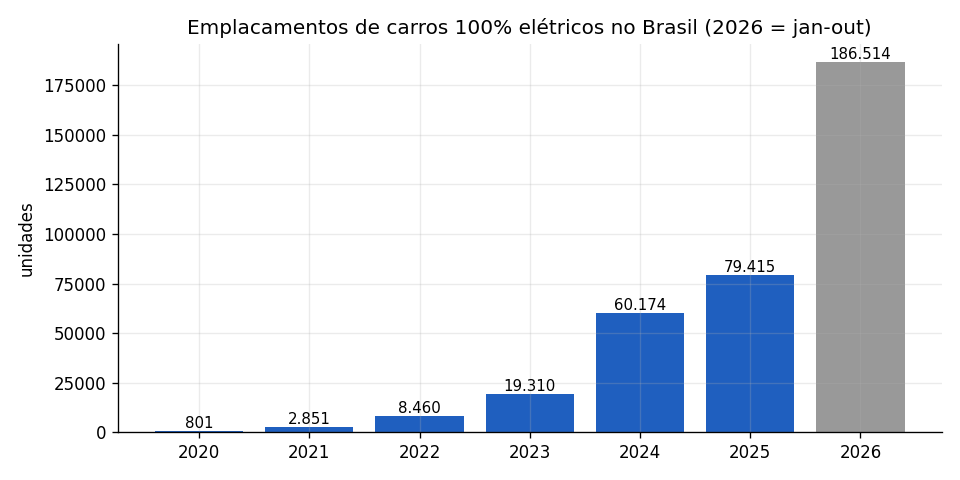
\includegraphics[width=0.49\linewidth]{figuras/01_tamanho_mercado.png}\hfill
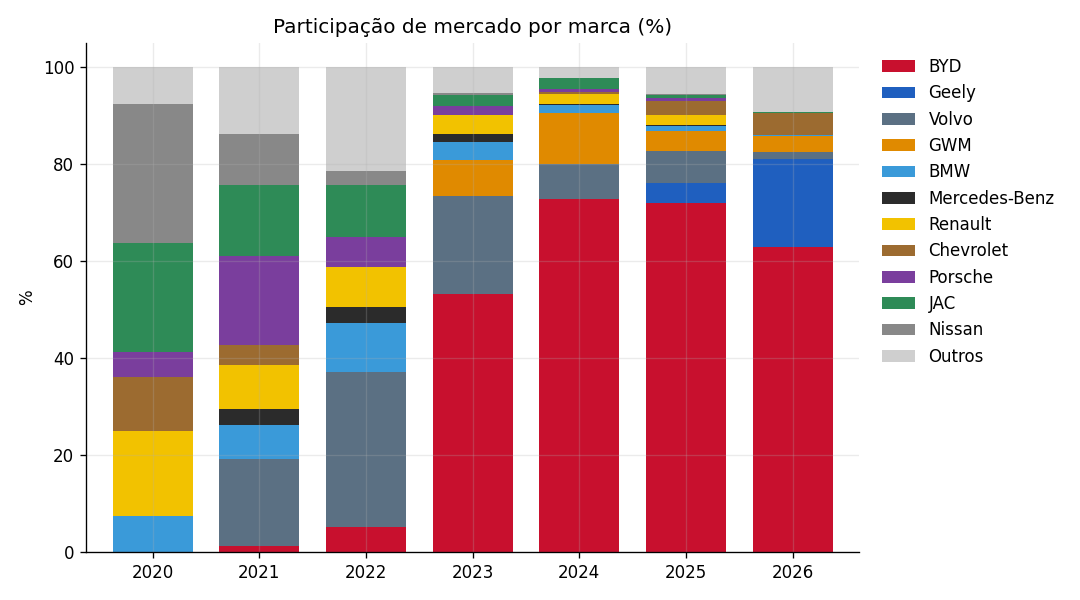
\includegraphics[width=0.49\linewidth]{figuras/02_participacao_marcas.png}
\caption{Tamanho do mercado (esq.) e participação por marca (dir.).}
\end{figure}

\begin{table}[H]
\centering\small
\begin{tabular}{@{}lrrlrrr@{}}
\toprule
Ano & Carros & HHI & Líder (CR1) & CR4 & Equiv. & Instab. (p.p.) \\
\midrule
2020$^*$ & 801    & 1.842 & Nissan 28,7\%  & 79,9\% & 5,4 & --- \\
2021$^*$ & 2.851  & 1.250 & Porsche 18,2\% & 61,4\% & 8,0 & 48,0 \\
2022$^*$ & 8.460  & 1.516 & Volvo 31,9\%   & 60,9\% & 6,6 & 35,9 \\
2023$^*$ & 19.310 & 3.343 & BYD 53,2\%     & 84,8\% & 3,0 & 55,4 \\
2024     & 60.174 & 5.478 & BYD 72,8\%     & 92,8\% & 1,8 & 23,6 \\
2025     & 79.415 & 5.274 & BYD 72,0\%     & 86,8\% & 1,9 & 11,2 \\
2026$^\dagger$ & 186.514 & 4.353 & BYD 63,0\% & 89,6\% & 2,3 & 21,2 \\
\bottomrule
\end{tabular}
\caption{Indicadores anuais. $^*$Divisão por marca estimada pelo grupo. $^\dagger$Janeiro a outubro.}
\end{table}

O setor passou por três fases:
\begin{enumerate}
  \item \textbf{Nicho premium (2020--2022).} Poucos milhares de carros por ano, divididos entre marcas importadas de luxo (Volvo, BMW, Porsche, Audi, Mercedes, Mini), que somavam mais da metade do mercado em 2022. Concentração baixa a moderada e liderança trocando de mãos todo ano.
  \item \textbf{Domínio da BYD (2023--2025).} A BYD entrou com o Dolphin abaixo de R\$\,150 mil (2023) e o Dolphin Mini por R\$\,115,8 mil (2024). Chegou a 73\% do mercado e o HHI passou de 5.000: o equivalente a menos de duas empresas do mesmo tamanho.
  \item \textbf{Desafio chinês (2026).} A Geely, com o EX2, virou a segunda força (18\% em 2026) e o HHI caiu para 4.353. As premium ficaram com cerca de 2\%.
\end{enumerate}

Entre 2024 e 2025 entraram 10 marcas novas (Ford, Volkswagen, Zeekr, GAC, Geely, Hyundai, Leapmotor, MG, Neta, Omoda Jaecoo), quase todas chinesas. Mesmo assim a concentração continuou alta: os entrantes ficaram com participações pequenas.

%=====================================================================
\section{Análise comparativa}

\textbf{Ao longo do tempo.} A tabela acima mostra a virada de 2023. Como os dados por marca de 2020--2023 são estimados, fizemos uma simulação de Monte Carlo com erro de até 30\% em cada estimativa: o HHI de 2022 fica entre 1.255 e 1.844 (não dá para afirmar se era baixo ou moderado), mas o de 2023 fica entre 3.244 e 3.457, sempre alto. A virada, portanto, não depende das estimativas.

\textbf{Com outros setores.} O mercado de elétricos é mais concentrado que o mercado automotivo como um todo (HHI $\approx$ 1.000), que os bancos ($\approx$ 1.000) e até que telefonia móvel ($\approx$ 3.100) e aviação doméstica ($\approx$ 3.300), setores com apenas três grandes empresas.

\textbf{Com definições de mercado diferentes.} O resultado depende de onde se traça a fronteira do mercado. Em 2026, o HHI é 4.553 considerando só elétricos, 2.020 incluindo os híbridos e 916 entre todos os automóveis; a BYD tem 64\%, 40\% e 10\% de cada um. O ``quase monopólio'' só vale na definição mais estreita, e os híbridos são um substituto próximo.

\begin{figure}[H]
\centering
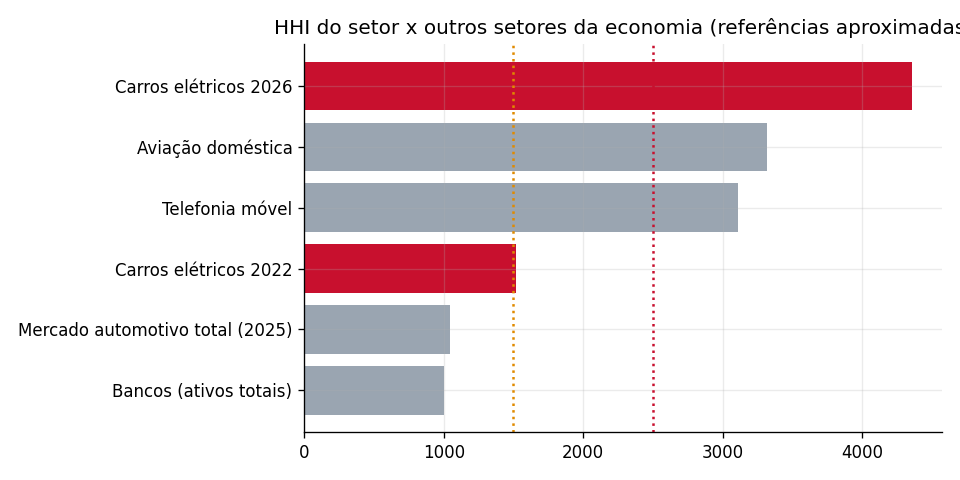
\includegraphics[width=0.49\linewidth]{figuras/04_comparacao_setores.png}\hfill
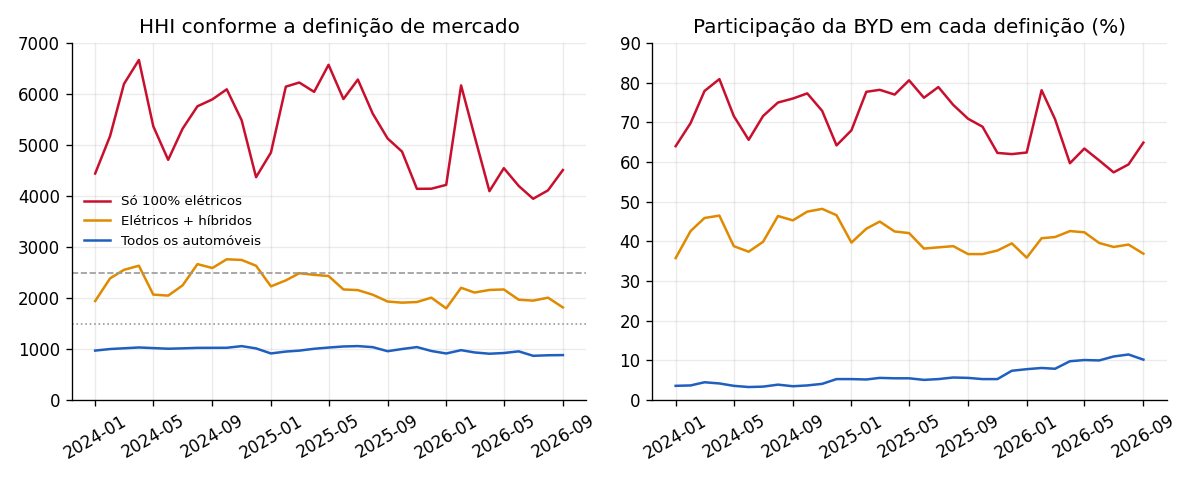
\includegraphics[width=0.49\linewidth]{figuras/10_definicoes_mercado.png}
\caption{HHI comparado a outros setores (esq.) e sob três definições de mercado (dir.).}
\end{figure}

%=====================================================================
\section{Tendências e padrões}

\textbf{Preços.} Na Tabela FIPE, entre jan/2024 e out/2026, o elétrico zero km mais barato caiu de R\$\,157 mil para R\$\,101 mil em valores reais; o preço mediano, de R\$\,294 mil para R\$\,230 mil; e o número de versões abaixo de R\$\,150 mil foi de 0 para 12. É o sinal mais claro de rivalidade: a disputa é na faixa de R\$\,100--120 mil (Dolphin Mini, Geely EX2, Renault Kwid E-Tech).

\textbf{Preço x características.} Numa regressão hedônica com 68 modelos ($R^2 = 0{,}87$), 10\% a mais de bateria valem 7,8\% no preço e 10\% a mais de potência, 3,5\%. Com as mesmas características, uma marca chinesa custa 26\% menos ($p<0{,}001$) e uma premium, 24\% mais. É a estratégia de liderança em custo medida nos dados.

\textbf{Grupos estratégicos.} Um agrupamento k-means por preço, bateria e potência encontra três grupos: entrada (8 modelos, mediana de R\$\,125 mil, 62\% chineses), intermediário (34 modelos, R\$\,232 mil, 59\% chineses) e premium (26 modelos, R\$\,543 mil, 27\% chineses). As chinesas disputam entre si as duas primeiras faixas e só enfrentam as tradicionais na terceira.

\begin{figure}[H]
\centering
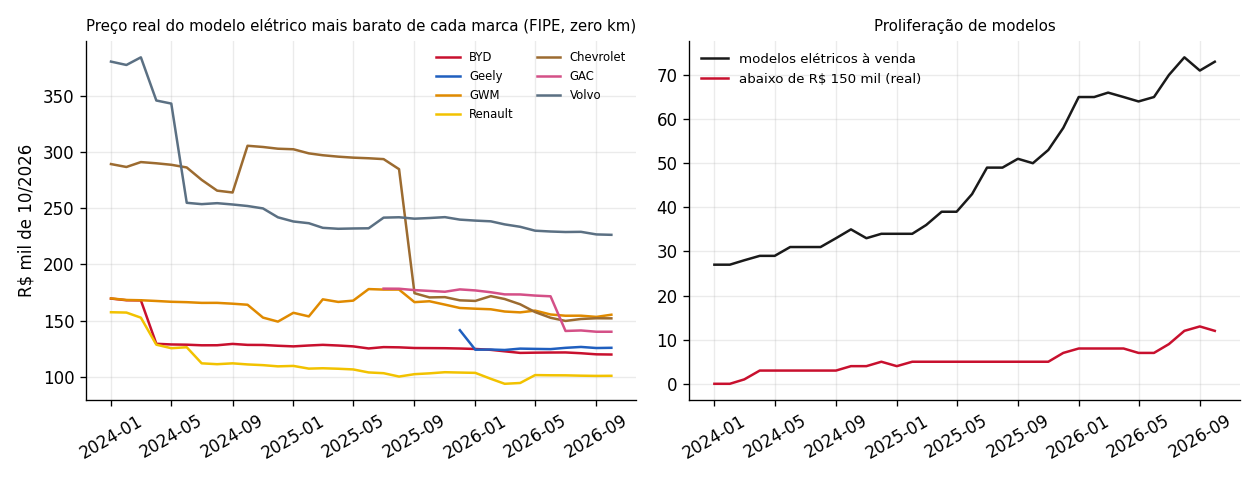
\includegraphics[width=0.49\linewidth]{figuras/15_precos_fipe.png}\hfill
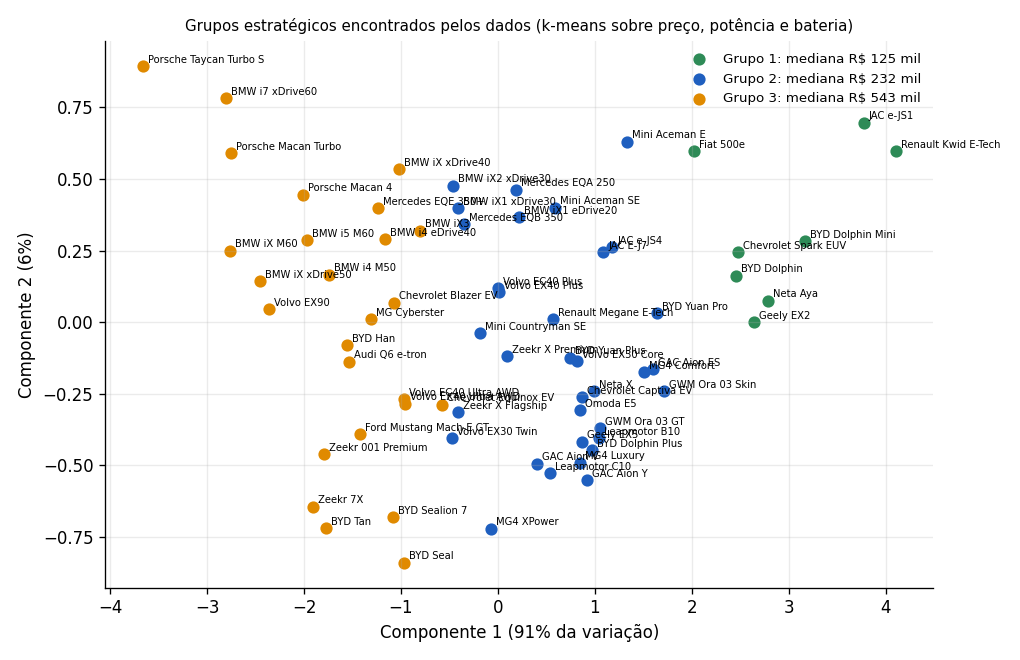
\includegraphics[width=0.49\linewidth]{figuras/17_grupos_estrategicos.png}
\caption{Preços reais na Tabela FIPE (esq.) e grupos estratégicos (dir.).}
\end{figure}

\textbf{Imposto de importação e estoque.} O imposto sobre elétricos voltou em degraus: 10\% (jan/2024), 18\% (jul/2024), 25\% (jul/2025) e 35\% (jul/2026). No Comex Stat, as importações disparam no mês anterior a cada alta (picos de 32 mil carros em jun/2024 e 48 mil em jun/2026) e caem de 4,5 a 7 vezes nos três meses seguintes: as marcas antecipam estoque. A China responde por 97\% das unidades importadas desde 2024.

\textbf{O que tirou participação da BYD.} Numa série temporal interrompida com os 34 meses de dados oficiais, controlando a tendência, a chegada do Geely EX2 em volume (nov/2025) está associada a uma queda de 10,1 p.p. na participação da BYD ($p = 0{,}001$). Nenhuma alta do imposto teve efeito estatisticamente significativo isolado, e um teste de quebra estrutural sem data informada aponta out/2025. A concorrência de produto pesou mais que a política tributária.

\begin{figure}[H]
\centering
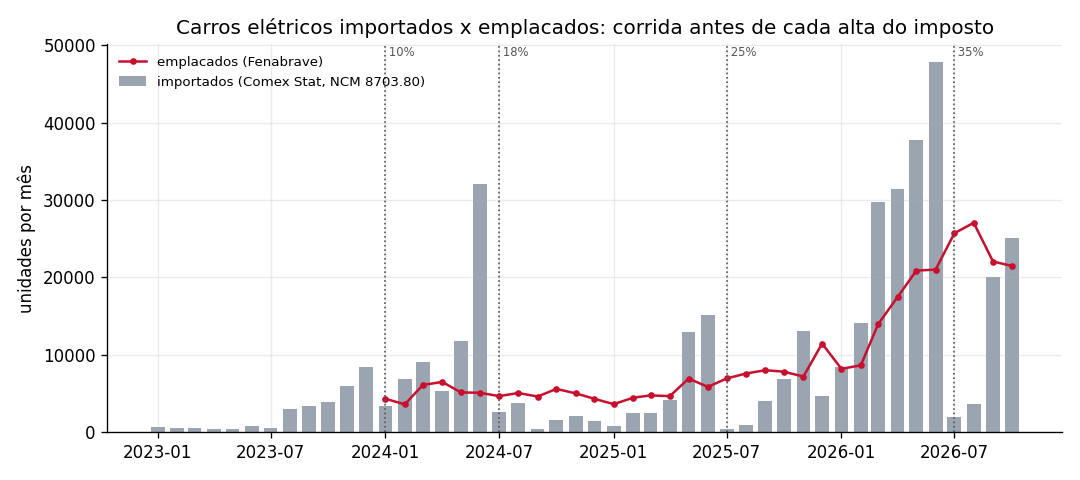
\includegraphics[width=0.49\linewidth]{figuras/13_importacoes_estoque.png}\hfill
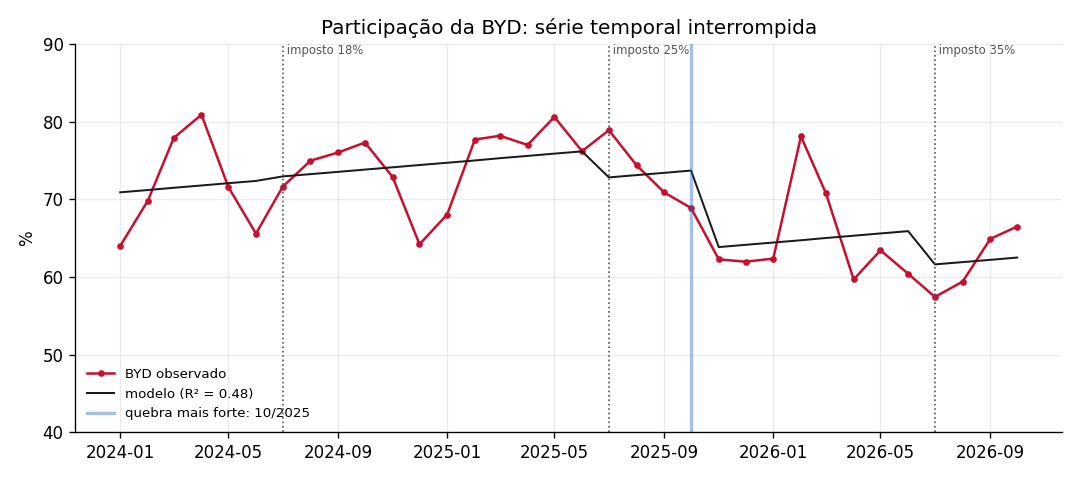
\includegraphics[width=0.49\linewidth]{figuras/12_serie_interrompida_byd.png}
\caption{Importações antes e depois de cada alta do imposto (esq.) e participação mensal da BYD com os eventos testados (dir.).}
\end{figure}

\textbf{Crescimento.} De 2024 a 2026 os emplacamentos cresceram em média 5,4\% ao mês (dobram a cada 13 meses). Um modelo de difusão de Bass mostra adoção movida por imitação, e não por propaganda, mas ainda não permite estimar o teto do mercado, porque a curva só acelera.

%=====================================================================
\section{Discussão: nível de rivalidade, desafios e oportunidades}
O setor combina \textbf{estrutura muito concentrada} com \textbf{rivalidade intensa em preço}. A concentração alta vem de uma única empresa com vantagem de custo (bateria própria e produção em escala), e não de um acordo entre poucas empresas. Pelas 5 Forças de Porter, de 2022 para 2026 a rivalidade e o poder dos compradores aumentaram (mais marcas e clientes comparando preço), enquanto a ameaça de entrada diminuiu com o imposto de 35\% e o custo de montar fábrica no país.

\begin{itemize}
  \item \textbf{Desafios:} guerra de preços apertando margens; imposto de 35\% para quem só importa; concorrência dos híbridos, que venderam mais que os elétricos em 2025; recarga pública limitada e juros altos no financiamento.
  \item \textbf{Oportunidades:} mercado que ainda dobra a cada ano; produção local (BYD em Camaçari, Geely com a Renault no Paraná) como forma de escapar do imposto e exportar para a América Latina; faixa intermediária de preço com menos concorrentes; frotas, locadoras e motoristas de aplicativo.
\end{itemize}

%=====================================================================
\section{O portal (protótipo)}
O portal (\texttt{portal/index.html}) roda direto no navegador e cobre os recursos sugeridos na proposta do trabalho:
\begin{itemize}
  \item \textbf{Dashboard personalizado:} o usuário escolhe o ano, a métrica (\% ou unidades), as marcas exibidas e quais painéis aparecem; as escolhas ficam salvas no navegador.
  \item \textbf{Visualizações interativas:} participação por marca, HHI e CR4, ranking com o status de cada dado, comparação com outros setores, preços, imposto e linha do tempo.
  \item \textbf{Análise avançada:} um simulador recalcula o HHI se uma marca tomar participação de outra ou se duas se fundirem; a aba de série mensal traz os resultados estatísticos da Seção 7; a aba estratégica tem as 5 Forças com notas ajustáveis, estratégias genéricas, SWOT, Mintzberg, Chandler e o modelo TAM.
  \item \textbf{Compartilhamento:} botões para copiar o resumo da análise e os dados em CSV.
  \item \textbf{Responsividade:} o layout se adapta a celular e segue o tema claro ou escuro do sistema.
\end{itemize}

%=====================================================================
\section{Limitações}
\begin{itemize}
  \item A divisão por marca de 2020 a 2023 é estimativa do grupo (só os totais são oficiais); a incerteza foi medida por Monte Carlo.
  \item A Fenabrave publica só as 15 maiores marcas por mês; outubro de 2026 tem só as 5 maiores.
  \item A NCM de importação inclui veículos elétricos pequenos que não são emplacados como automóvel, então importações e emplacamentos não fecham exatamente.
  \item Potência, bateria e datas de produção local foram compiladas de fichas técnicas e notícias.
  \item Com 34 meses e eventos próximos entre si, os testes estatísticos indicam a direção dos efeitos com mais segurança do que o tamanho.
\end{itemize}

%=====================================================================
\section*{Referências}
\small
\begin{itemize}
  \item ABVE --- Associação Brasileira do Veículo Elétrico. Balanços anuais de emplacamentos.
  \item Banco Central do Brasil. Sistema Gerenciador de Séries Temporais (séries 20749, 4189, 433, 3698).
  \item CADE. Guia para análise de atos de concentração horizontal, 2016.
  \item Fenabrave. Informativo mensal de emplacamentos, jan/2024 a out/2026.
  \item FIPE. Tabela FIPE de preços médios de veículos.
  \item Hymer, S.; Pashigian, P. Turnover of firms as a measure of market behavior. \emph{Review of Economics and Statistics}, 1962.
  \item MDIC. Comex Stat --- estatísticas de comércio exterior.
  \item Porter, M. \emph{Estratégia competitiva}. Rio de Janeiro: Campus, 1986.
\end{itemize}

\end{document}
